
\begin{figure}
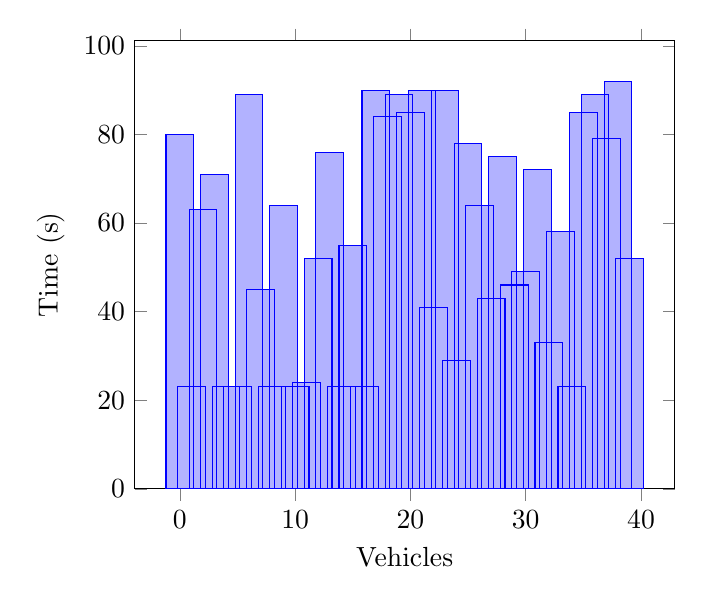
\begin{tikzpicture}
\begin{axis}[
legend style={anchor=west},
xlabel=Vehicles,
ylabel=Time (s),
ymin=0,
ybar,
]
\addplot coordinates {
(0, 80)
(1, 23)
(2, 63)
(3, 71)
(4, 23)
(5, 23)
(6, 89)
(7, 45)
(8, 23)
(9, 64)
(10, 23)
(11, 24)
(12, 52)
(13, 76)
(14, 23)
(15, 55)
(16, 23)
(17, 90)
(18, 84)
(19, 89)
(20, 85)
(21, 90)
(22, 41)
(23, 90)
(24, 29)
(25, 78)
(26, 64)
(27, 43)
(28, 75)
(29, 46)
(30, 49)
(31, 72)
(32, 33)
(33, 58)
(34, 23)
(35, 85)
(36, 89)
(37, 79)
(38, 92)
(39, 52)
};

\end{axis}
\end{tikzpicture}
\label{tik:100:10}
\caption{100 percent diving with GSC on route $10$}
\end{figure}
